\subsection{Least Squares Normalizado}

Nas simula��es, procuramos avaliar o comportamento do sistema para as seguintes condi��es:
%
\begin{enumerate*}[label=(\roman*)]
\item condi��o inicial $\theta(0)$;
\item sinal de refer�ncia $r(t)$;
\item matriz de ganho inicial $P_0 = P(0)$.
\end{enumerate*}

Apresentaremos os resultados obtidos atrav�s de simula��es no ambiente \HI{\texttt{Matlab/Simulink}} e os discutiremos na pr�xima se��o.

%%%%%%%%%%%%%%%%%%%%%%%%%%%%%%%%%%%%%%%%%%%%%%%%%%%%%%%%%%%%%%%%%%%%%%%%%%%%%%%%%%%%%%%%%%%%%%%%%%%%%%%%%
\subsection{Simula��o \#1}% 1 ordem

Inicialmente, desejamos verificar o comportamento do sistema para varia��es no
sinal de refer�ncia $r(t)$ para podermos analisar a influ�ncia da persist�ncia
de excita��o.

%\bigskip%
%Par�metros e condi��es iniciais :
%
\begin{align*}
  y &= \frac{1}{s+2}u\,,  &  \Lambda &= \frac{1}{s+1}\,, & \theta(0) &= 0\,, \\
  P_0 &= 5\,I_2\,, & r &= \HI{1, $1+5\textrm{sin}(t)$}\, \,.
\end{align*}

\bigskip%
\begin{figure}[H]
  \centering
  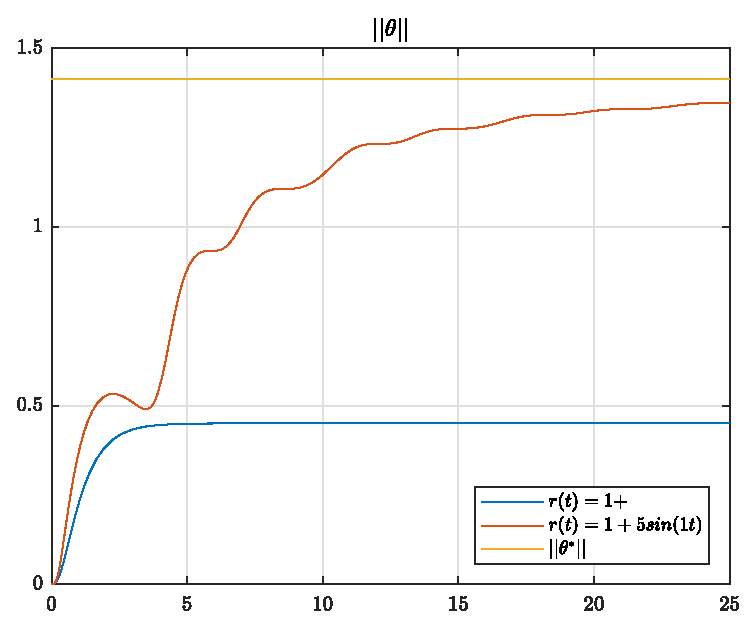
\includegraphics[width=12.5cm]{figs/ls/modtheta/sim01_r1r2.eps} \\[2mm]
\end{figure}

\begin{figure}[H]
  \centering
  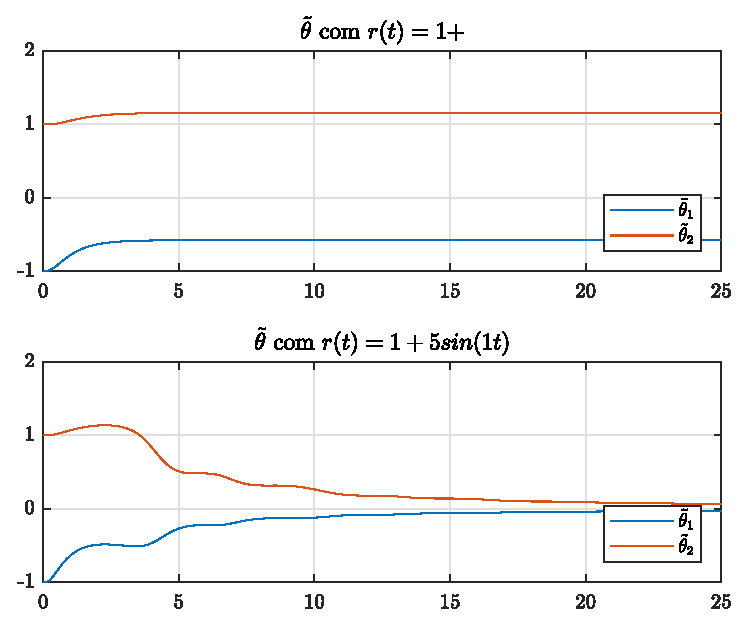
\includegraphics[width=12.5cm]{figs/ls/tiltheta/sim01_r1r2.eps} 
\end{figure}


\begin{figure}[H]
  \centering
  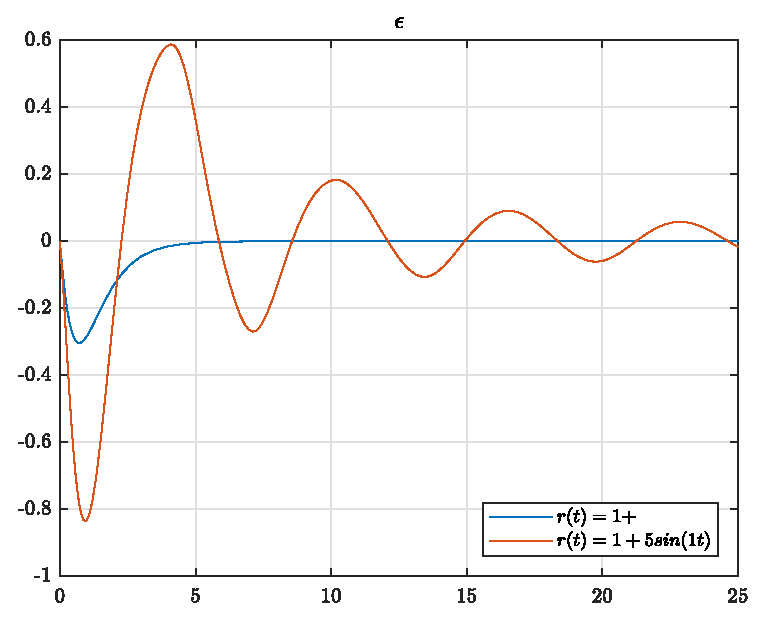
\includegraphics[width=12.5cm]{figs/ls/epsilon/sim01_r1r2.eps} 
\end{figure}

\newpage%

%%%%%%%%%%%%%%%%%%%%%%%%%%%%%%%%%%%%%%%%%%%%%%%%%%%%%%%%%%%%%%%%%%%%%%%%%%%%%%%%%%%%%%%%%%%%%%%%%%%%%%%%%
% 2 ordem
\begin{align*}
  y &= \frac{s+1}{s^2+4s+4}u\,,  &  \Lambda &= \frac{1}{s^2+2s+1}\,, & \theta(0)
  &= 0\,,\\
  P_0 &= 10 \, I_4 \,, & r &= \HI{$30\textrm{sin}(w_1 \, t)$} e
  \HI{$30\textrm{sin}(w_1 \, t)+25\textrm{sin}(w_2 \, t)$}\, \,.
\end{align*}

\bigskip%
\begin{figure}[H]
  \centering
  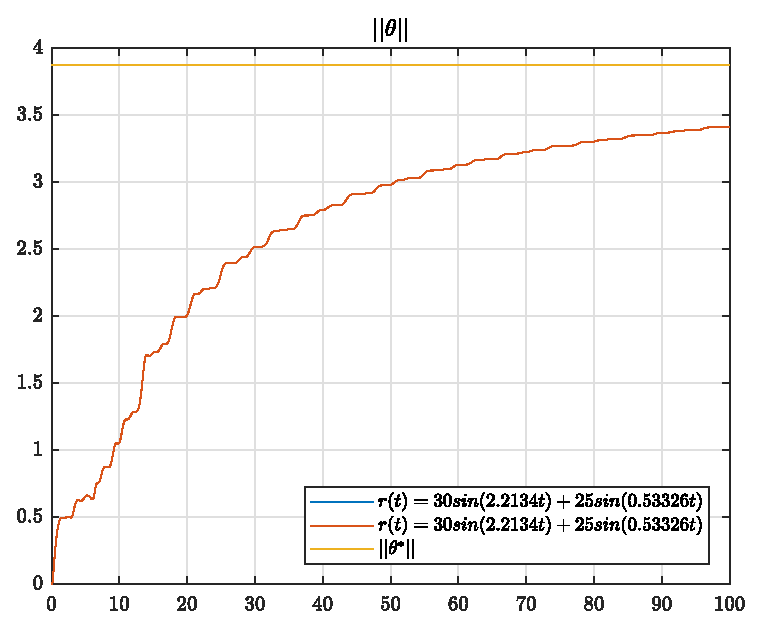
\includegraphics[width=12.5cm]{figs/ls/modtheta/sim02_r1r2.eps} \\[2mm]
\end{figure}

\begin{figure}[H]
  \centering
  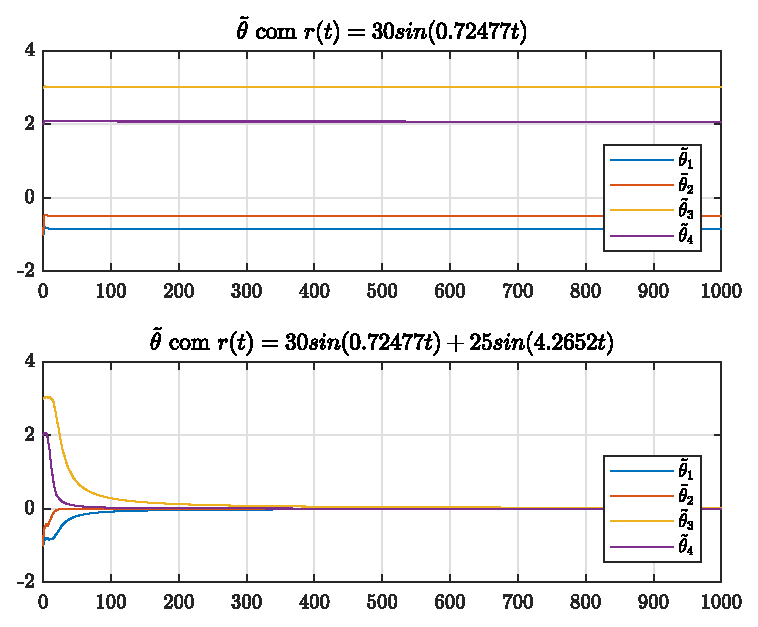
\includegraphics[width=12.5cm]{figs/ls/tiltheta/sim02_r1r2.eps} 
\end{figure}


\begin{figure}[H]
  \centering
  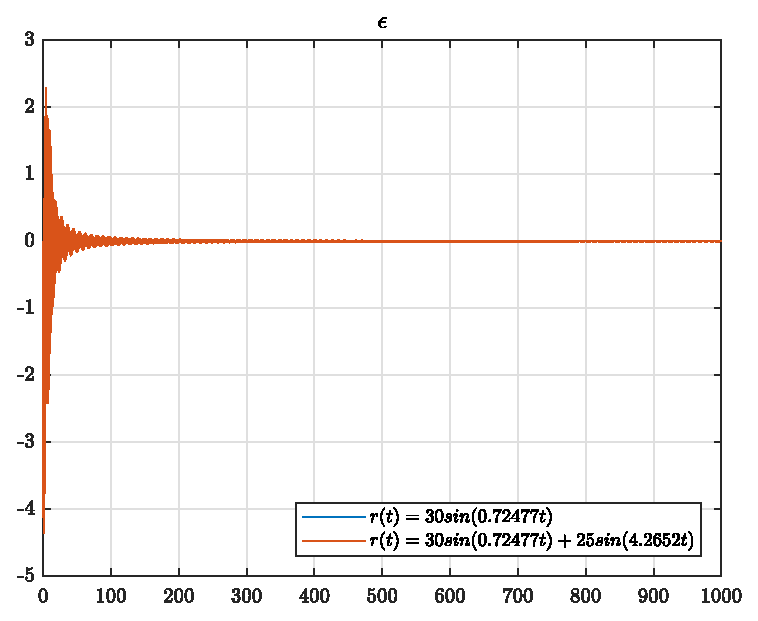
\includegraphics[width=12.5cm]{figs/ls/epsilon/sim02_r1r2.eps} 
\end{figure}

\newpage%

%%%%%%%%%%%%%%%%%%%%%%%%%%%%%%%%%%%%%%%%%%%%%%%%%%%%%%%%%%%%%%%%%%%%%%%%%%%%%%%%%%%%%%%%%%%%%%%%%%%%%%%%%
% 3 ordem
\begin{align*}
  y &= \frac{s^2+s+1}{s^3+s^2+s+1}u\,,  &  \Lambda &=
  \frac{1}{s^3+3s^2+3s+1}\,, & \theta(0) &= 0\,,\\
  P_0 &= 10 \, I_6 \,, & r &= \HI{$10\textrm{sin}(w_1 \, t) + 5\textrm{sin}(w_2 \, t)$} e \HI{$\sum^{5}_{i=1} a_i \, \textrm{sin}(w_i \, t)$}\, \,.
\end{align*}

\bigskip%
\begin{figure}[H]
  \centering
  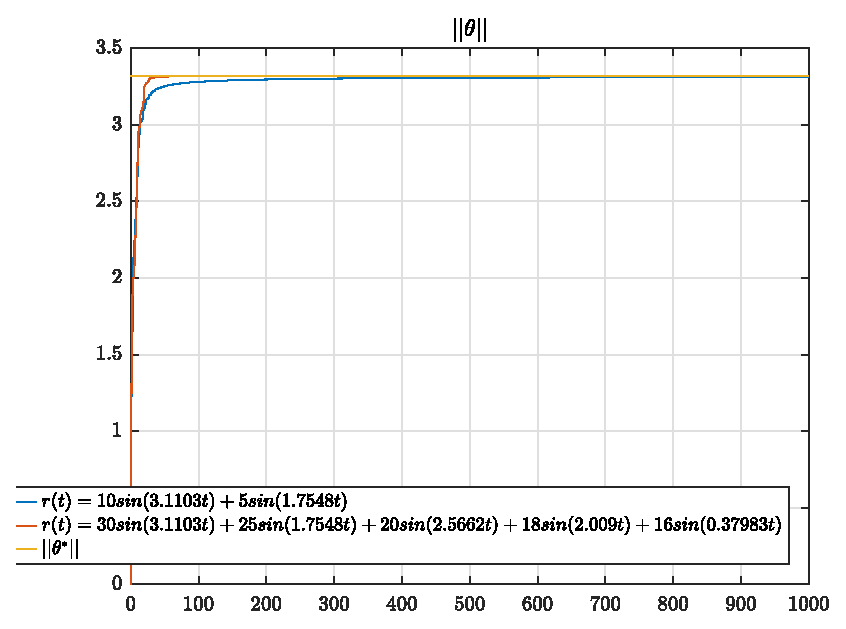
\includegraphics[width=12.5cm]{figs/ls/modtheta/sim03_r1r2.eps} \\[2mm]
\end{figure}

\begin{figure}[H]
  \centering
  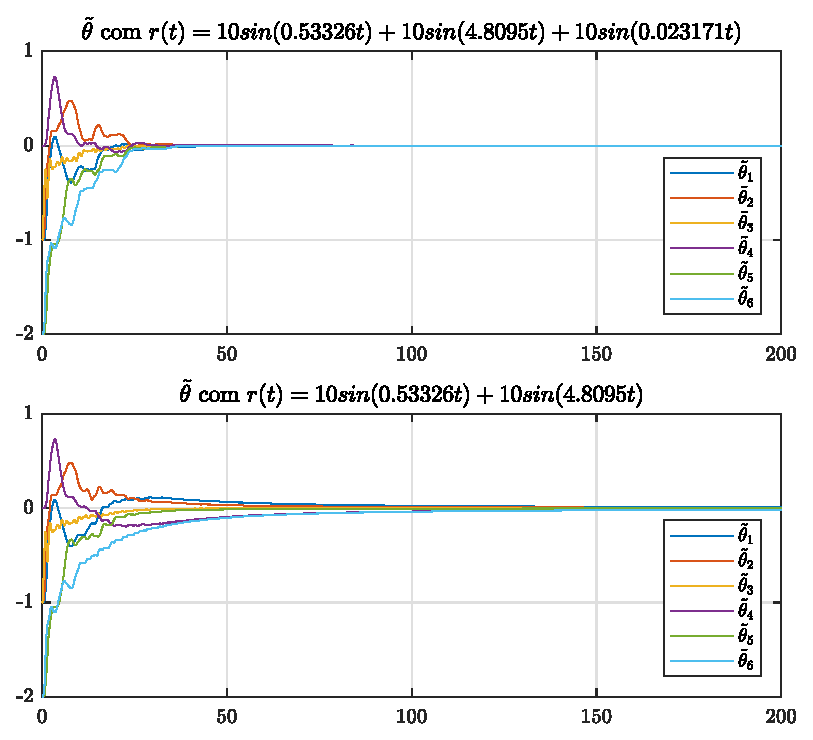
\includegraphics[width=12.5cm]{figs/ls/tiltheta/sim03_r1r2.eps} 
\end{figure}


\begin{figure}[H]
  \centering
  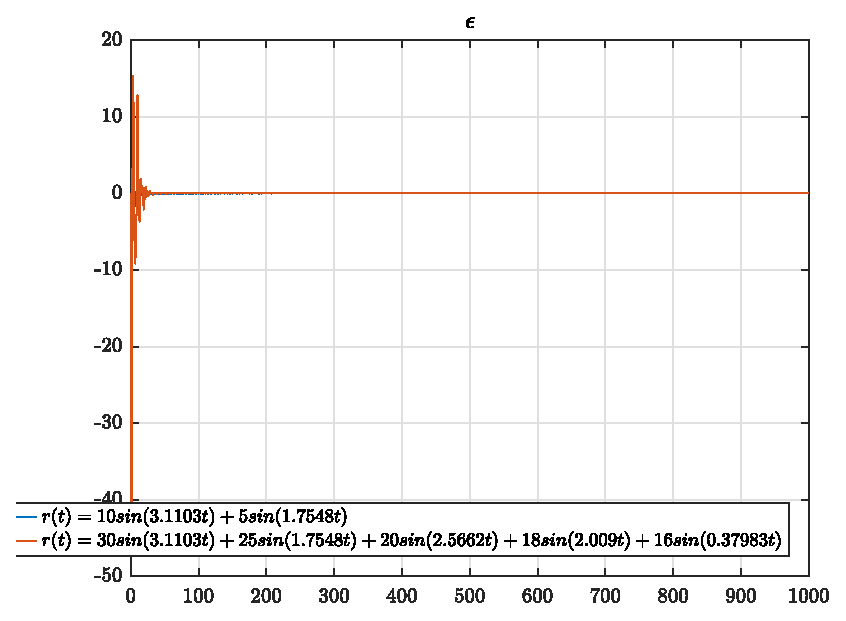
\includegraphics[width=12.5cm]{figs/ls/epsilon/sim03_r1r2.eps} 
\end{figure}

%%%%%%%%%%%%%%%%%%%%%%%%%%%%%%%%%%%%%%%%%%%%%%%%%%%%%%%%%%%%%%%%%%%%%%%%%%%%%%%%%%%%%%%%%%%%%%%%%%%%%%%%%
\subsection{Simula��o \#2}% 1 ordem

Na segunda simula��o, observamos o comportamento do sistema para varia��es do ganho inicial $P_0$:

\begin{align*}
  y &= \frac{1}{s+2}u\,,  &  \Lambda &= \frac{1}{s+1}\,, & \theta(0) &= 0\,, \\
  P_0 &= \HI{5, 10} I_2 \,, & r &= 1 + 5\,\textrm{sin}(t)\, \,.
\end{align*}

\bigskip%
\begin{figure}[H]
  \centering
  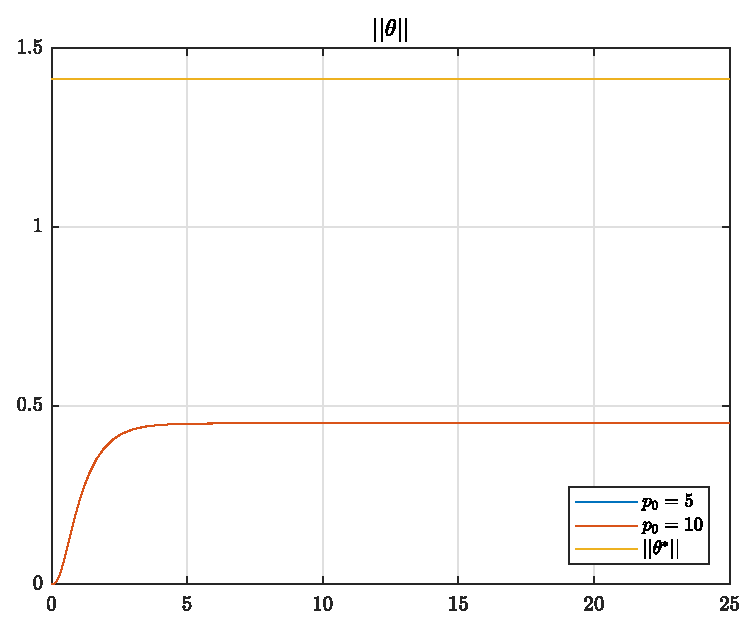
\includegraphics[width=12.5cm]{figs/ls/modtheta/sim01_p5p10.eps} \\[2mm]
\end{figure}

\begin{figure}[H]
  \centering
  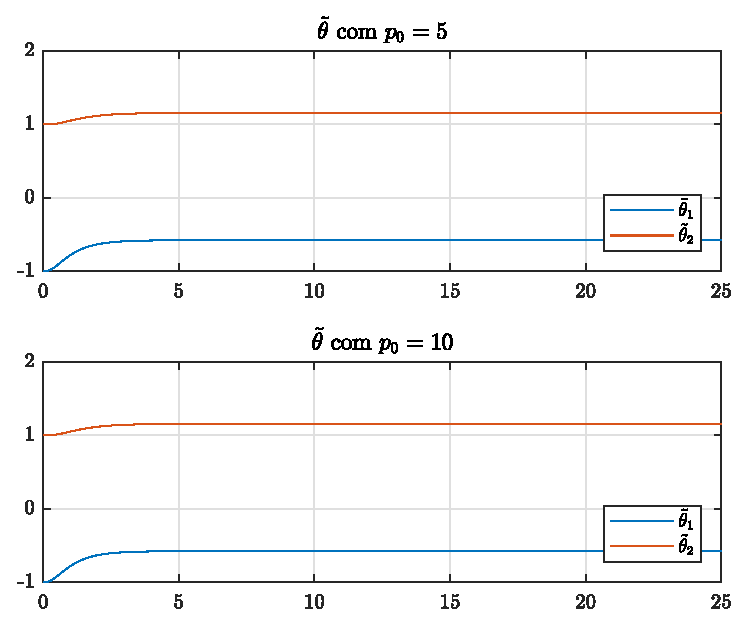
\includegraphics[width=12.5cm]{figs/ls/tiltheta/sim01_p5p10.eps} 
\end{figure}


\begin{figure}[H]
  \centering
  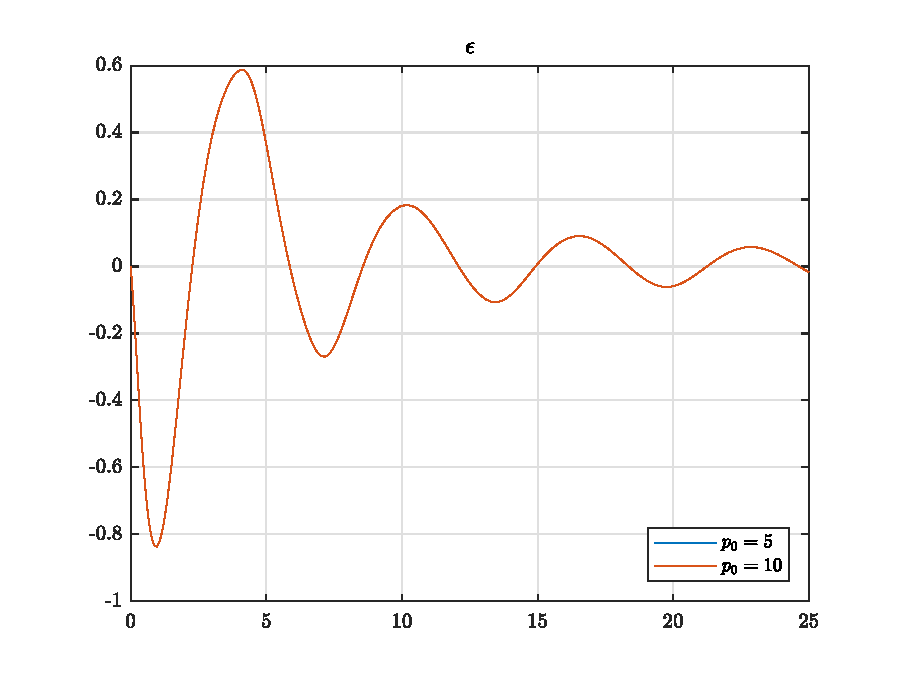
\includegraphics[width=12.5cm]{figs/ls/epsilon/sim01_p5p10.eps} 
\end{figure}

\newpage%

%%%%%%%%%%%%%%%%%%%%%%%%%%%%%%%%%%%%%%%%%%%%%%%%%%%%%%%%%%%%%%%%%%%%%%%%%%%%%%%%%%%%%%%%%%%%%%%%%%%%%%%%%
% 2 ordem
\begin{align*}
  y &= \frac{s+1}{s^2+4s+4}u\,,  &  \Lambda &= \frac{1}{s^2+2s+1}\,, & \theta(0)
  &= 0\,,\\
  P_0 &= \HI{10,100} I_4 \,, & r &=
  30\textrm{sin}(w_1\,t)+25\textrm{sin}(w_2\,t) \,.
\end{align*}

\bigskip%
\begin{figure}[H]
  \centering
  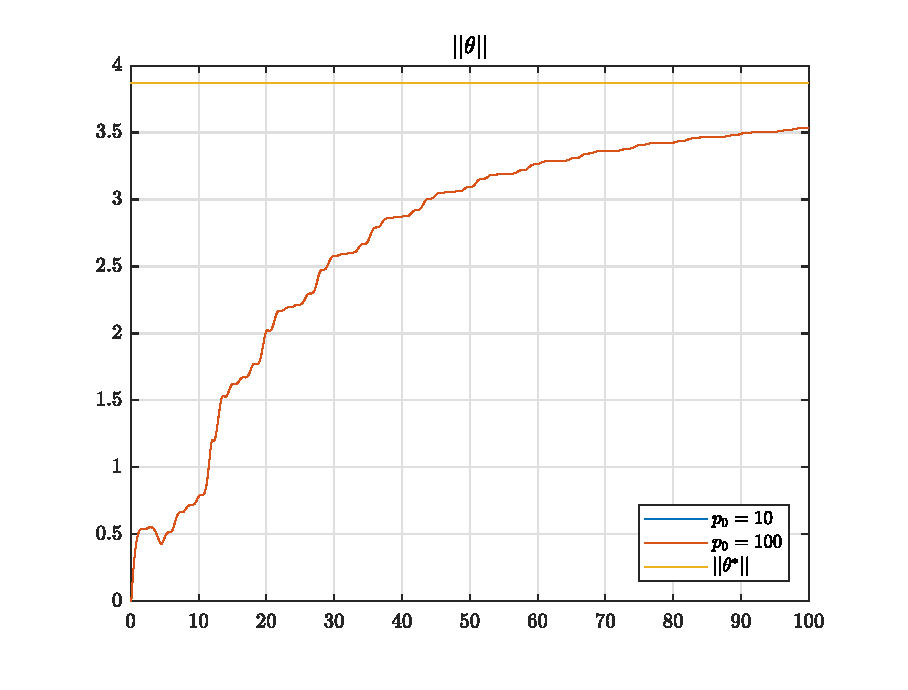
\includegraphics[width=12.5cm]{figs/ls/modtheta/sim02_p10p100.eps}
  \\[2mm]
\end{figure}

\begin{figure}[H]
  \centering
  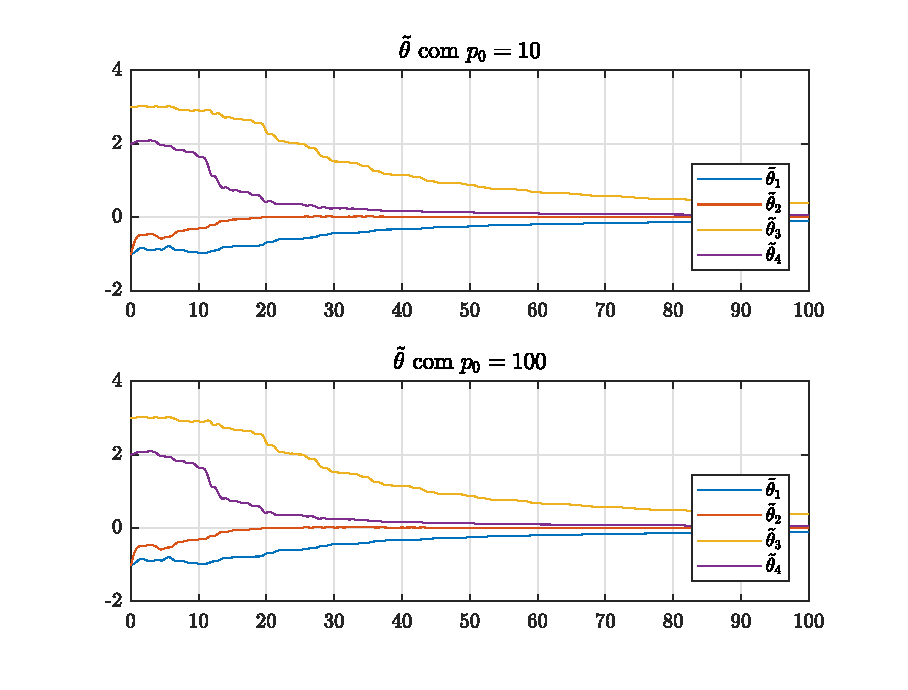
\includegraphics[width=12.5cm]{figs/ls/tiltheta/sim02_p10p100.eps} 
\end{figure}


\begin{figure}[H]
  \centering
  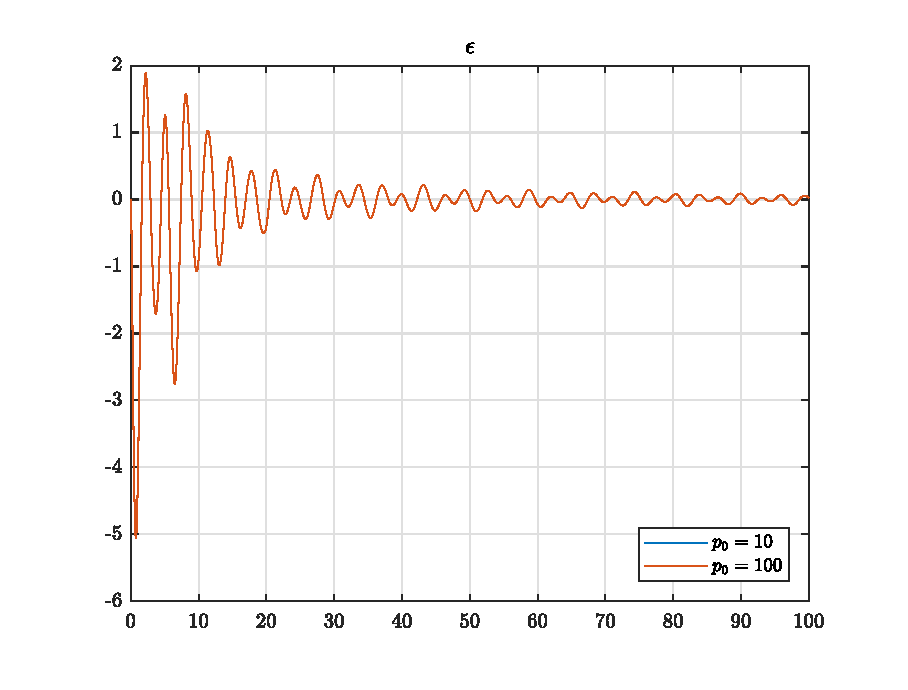
\includegraphics[width=12.5cm]{figs/ls/epsilon/sim02_p10p100.eps} 
\end{figure}

\newpage%

%%%%%%%%%%%%%%%%%%%%%%%%%%%%%%%%%%%%%%%%%%%%%%%%%%%%%%%%%%%%%%%%%%%%%%%%%%%%%%%%%%%%%%%%%%%%%%%%%%%%%%%%%
% 3 ordem
\begin{align*}
  y &= \frac{s^2+s+1}{s^3+s^2+s+1}u\,,  &  \Lambda &=
  \frac{1}{s^3+3s^2+3s+1}\,, & \theta(0) &= 0\,,\\
  P_0 &= \HI{10,100} I_6 \,, & r &= 10\textrm{sin}(w_1\,t)+5\textrm{sin}(w_2\,t)\,.
\end{align*}

\bigskip%
\begin{figure}[H]
  \centering
  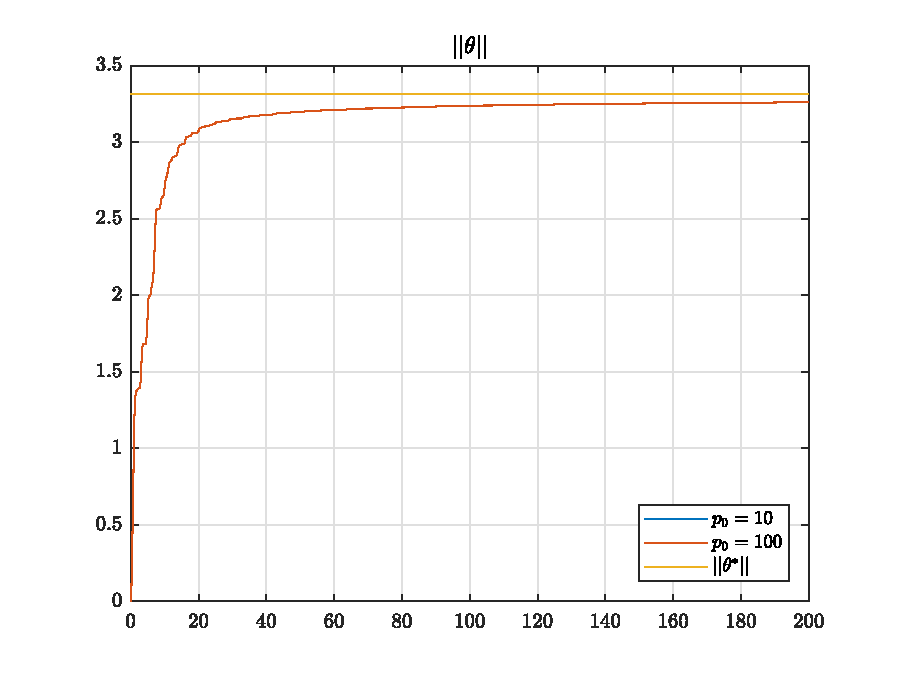
\includegraphics[width=12.5cm]{figs/ls/modtheta/sim03_p10p100.eps} \\[2mm]
\end{figure}

\begin{figure}[H]
  \centering
  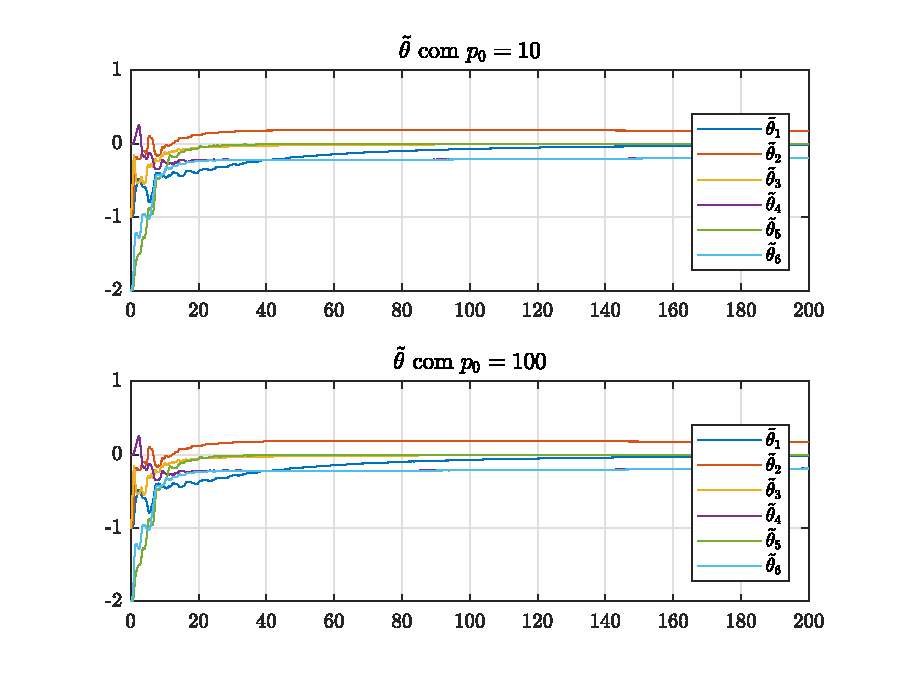
\includegraphics[width=12.5cm]{figs/ls/tiltheta/sim03_p10p100.eps} 
\end{figure}


\begin{figure}[H]
  \centering
  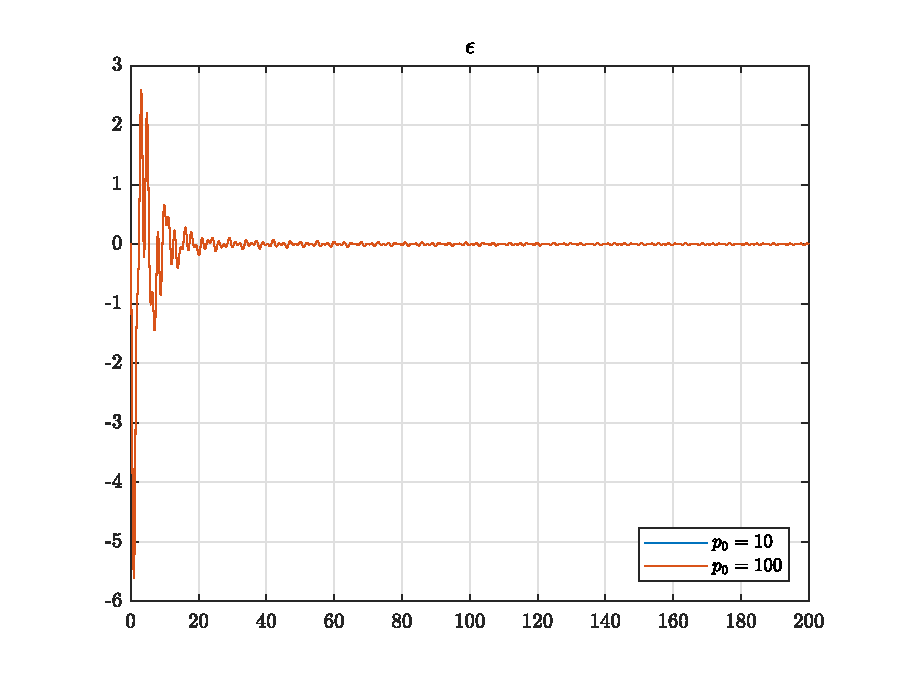
\includegraphics[width=12.5cm]{figs/ls/epsilon/sim03_p10p100.eps} 
\end{figure}

%%%%%%%%%%%%%%%%%%%%%%%%%%%%%%%%%%%%%%%%%%%%%%%%%%%%%%%%%%%%%%%%%%%%%%%%%%%%%%%%%%%%%%%%%%%%%%%%%%%%%%%%%
\subsection{Simula��o \#3} % 1 ordem

Na terceira simula��o, observamos o comportamento do sistema para varia��es nas
condi��es iniciais do vetor de par�metros estimados $\theta$.

\begin{align*}
  y &= \frac{1}{s+2}u\,,  &  \Lambda &= \frac{1}{s+1}\,, & \theta(0)
  &= \HI{0, 1}\,,\\
  P_0 &= 5 I_2 \,, & r &= 1+5\textrm{sin}(t) \,.
\end{align*}

\bigskip%
\begin{figure}[H]
  \centering
  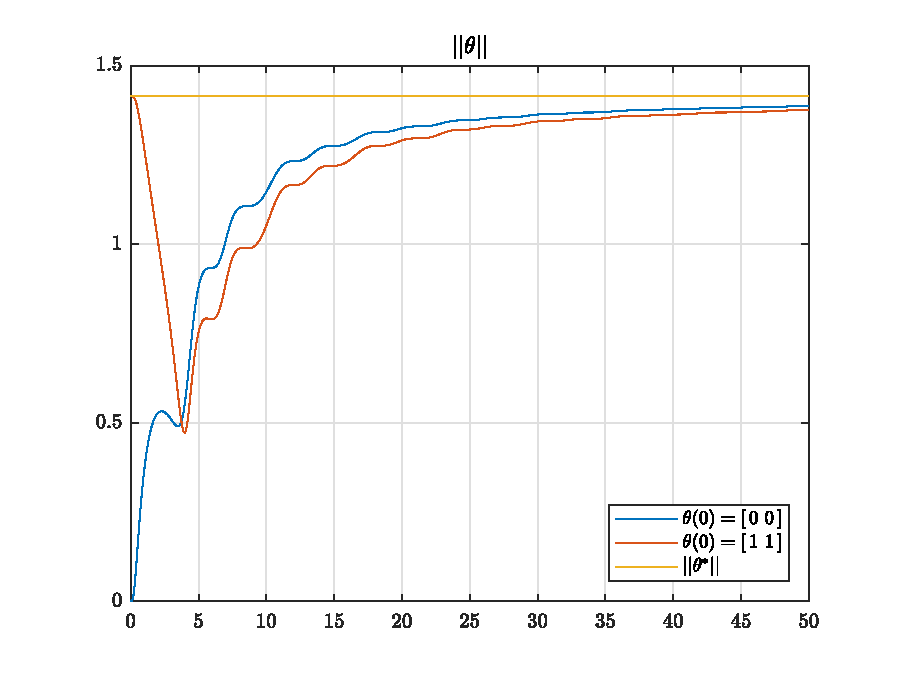
\includegraphics[width=12.5cm]{figs/ls/modtheta/sim01_theta01theta02.eps}
  \\[2mm]
\end{figure}

\begin{figure}[H]
  \centering
  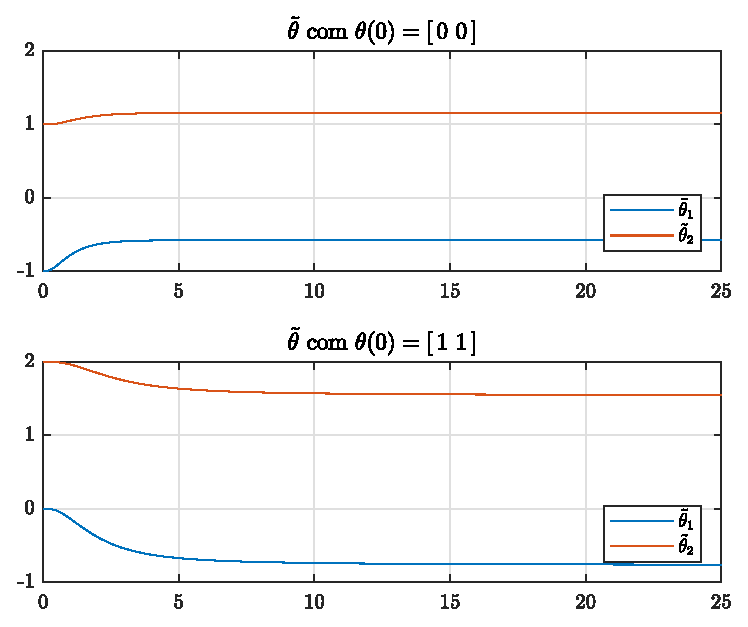
\includegraphics[width=12.5cm]{figs/ls/tiltheta/sim01_theta01theta02.eps} 
\end{figure}


\begin{figure}[H]
  \centering
  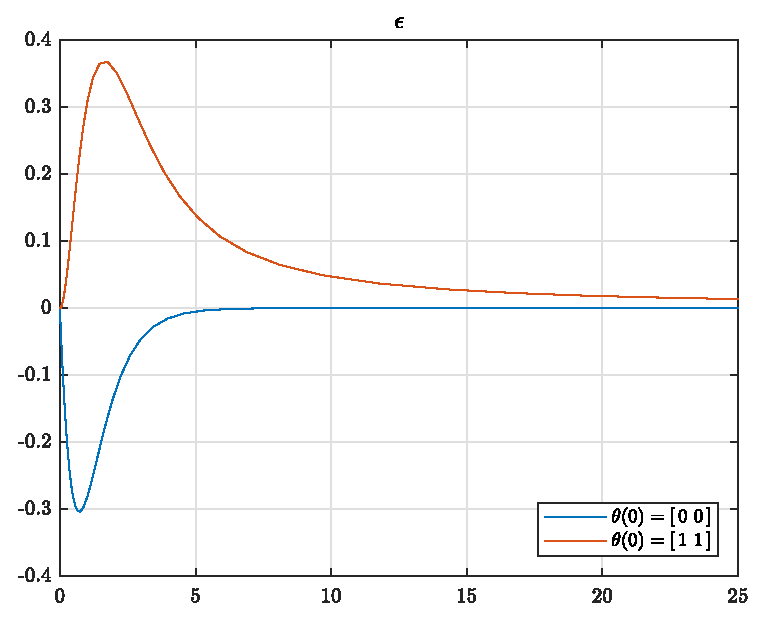
\includegraphics[width=12.5cm]{figs/ls/epsilon/sim01_theta01theta02.eps} 
\end{figure}

\newpage%

%%%%%%%%%%%%%%%%%%%%%%%%%%%%%%%%%%%%%%%%%%%%%%%%%%%%%%%%%%%%%%%%%%%%%%%%%%%%%%%%%%%%%%%%%%%%%%%%%%%%%%%%%
% 2 ordem
\begin{align*}
  y &= \frac{s+1}{s^2+4s+4}u\,,  &  \Lambda &= \frac{1}{s^2+2s+1}\,, & \theta(0)
  &= \HI{0, 1}\,,\\
  P_0 &= 10\,I_4 \,, & r &= 30\textrm{sin}(w_1\,t)+25\textrm{sin}(w_2\,t)\,.
\end{align*}

\bigskip%
\begin{figure}[H]
  \centering
  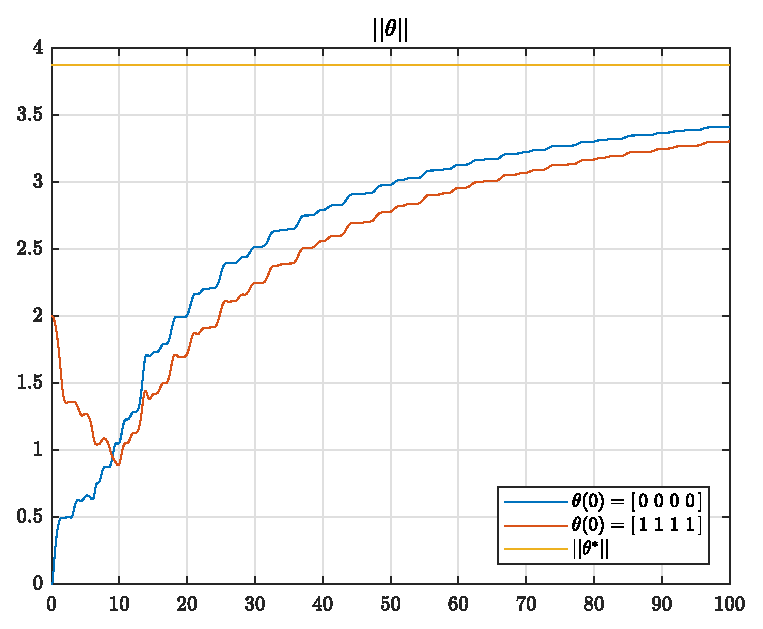
\includegraphics[width=12.5cm]{figs/ls/modtheta/sim02_theta01theta02.eps}
  \\[2mm]
\end{figure}

\begin{figure}[H]
  \centering
  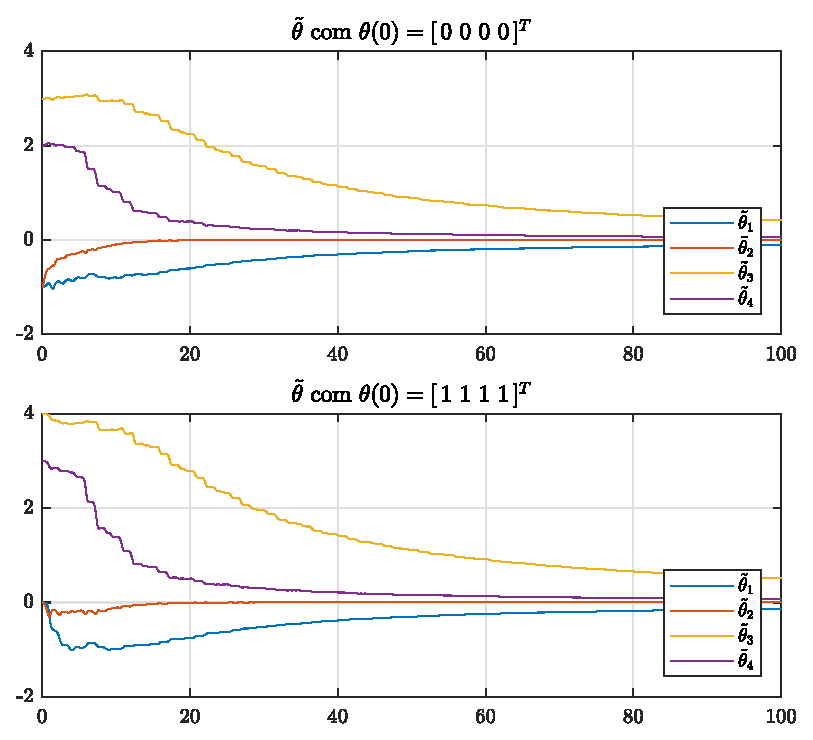
\includegraphics[width=12.5cm]{figs/ls/tiltheta/sim02_theta01theta02.eps} 
\end{figure}


\begin{figure}[H]
  \centering
  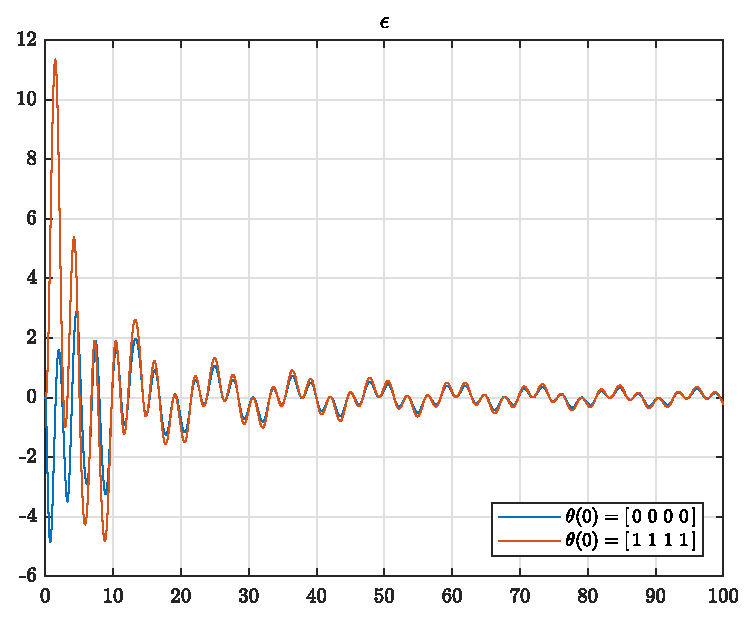
\includegraphics[width=12.5cm]{figs/ls/epsilon/sim02_theta01theta02.eps} 
\end{figure}

\newpage%

%%%%%%%%%%%%%%%%%%%%%%%%%%%%%%%%%%%%%%%%%%%%%%%%%%%%%%%%%%%%%%%%%%%%%%%%%%%%%%%%%%%%%%%%%%%%%%%%%%%%%%%%%
% 3 ordem
\begin{align*}
  y &= \frac{s^2+s+1}{s^3+s^2+s+1}u\,,  &  \Lambda &=
  \frac{1}{s^3+3s^2+3s+1}\,, & \theta(0) &= \HI{0, 1}\,,\\
  P_0 &= 10\,I_6 \,, & r &= 10\textrm{sin}(w_1\,t)+5\textrm{sin}(w_2\,t)\,.
\end{align*}

\bigskip%
\begin{figure}[H]
  \centering
  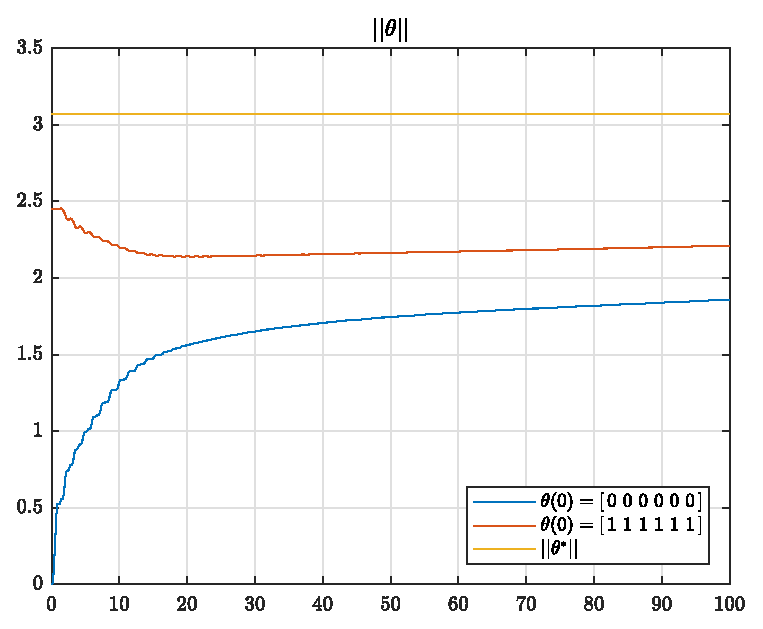
\includegraphics[width=12.5cm]{figs/ls/modtheta/sim03_theta01theta02.eps} \\[2mm]
\end{figure}

\begin{figure}[H]
  \centering
  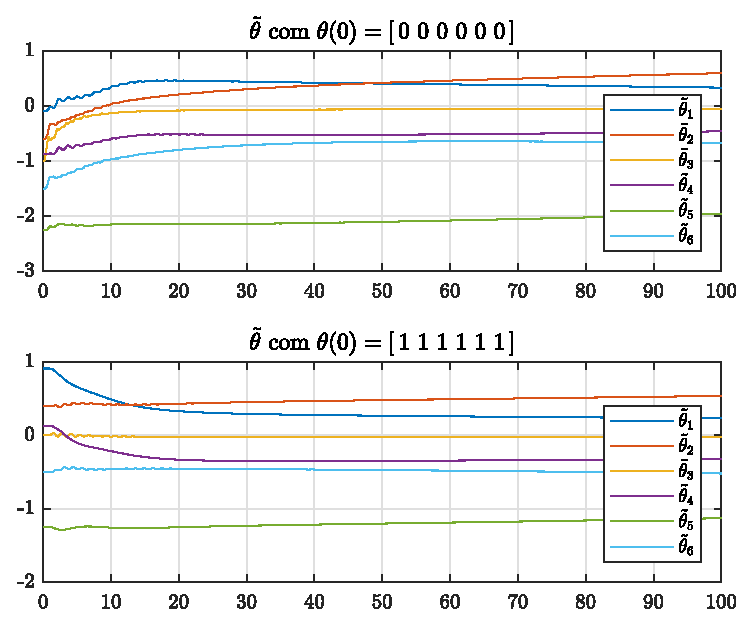
\includegraphics[width=12.5cm]{figs/ls/tiltheta/sim03_theta01theta02.eps} 
\end{figure}

\begin{figure}[H]
  \centering
  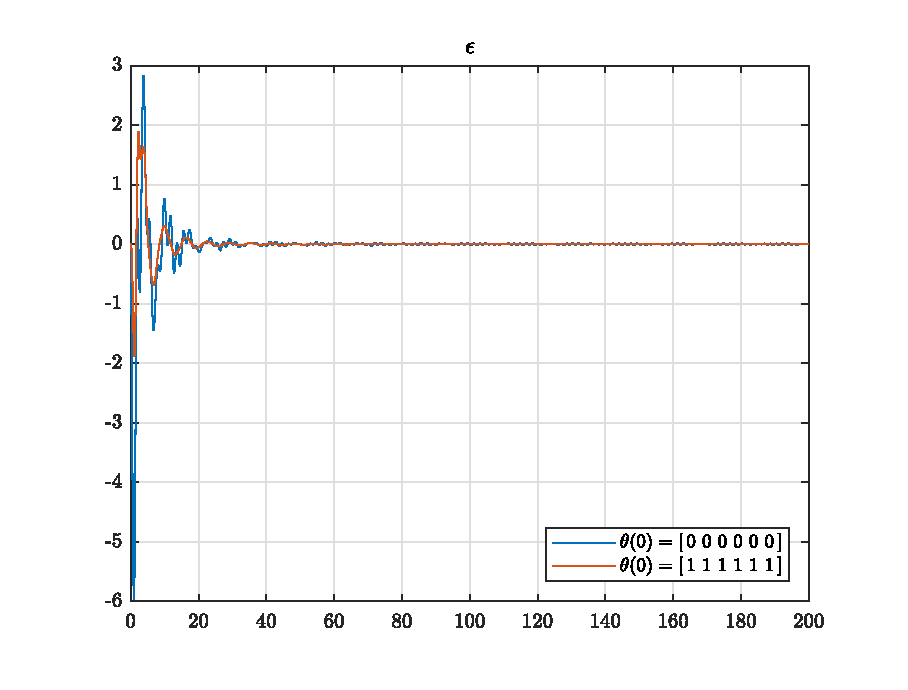
\includegraphics[width=12.5cm]{figs/ls/epsilon/sim03_theta01theta02.eps} 
\end{figure}
%---------------------------------------------------------------------